\chapter{Návrh riešenia}

\section{Metóda merania hĺbky pamäte samorganizujúcich sa máp}

\subsection{Trénovacie dáta}
Trénovacie sekvencie pozostávajú zo sekvencie písmen anglickej abecedy (26 písmen).
Spoločnou vlasťnosťou týchto trénovacích množín je, že sú tvorené/generované určitým nenáhodným spôsobom (obsahujú napríklad opakujúce sa podsekvencie)
a teda môžeme na nich natrénovať rekurentné neurónové siete. Inými slovami dokážu v nich 
neurónové siete zachytiť určité vzory správania.
Samotné vstupy (trénovacie príklady) pre sieť sú zakódované jednotlivé písmená z trénovacej sekvencie.
Keďže neurónové siete vedia pracovať iba s číselnými hodnotami, jednotlivé písmená zo 
vstupnej sekvencie kódujeme počas trénovania do 26 prvkového vektora, 
ktorého prvky sú nuly a jednotka (pre každé písmeno je jednotka na unikátnej pozícii).
Napríklad písmeno A bude reprezentované vektorom
$[1, 0, 0, 0, 0, 0, 0, 0, 0, 0, 0, 0, 0, 0, 0, 0, 0, 0, 0, 0, 0, 0, 0, 0]$
Tento spôsob reprezentácie vstupov pre sieť je jednoduchý a efektívny.

\subsection{Spôsob uchovávania informácii v SOM}
Na to aby sme boli schopný odmerať pamäťovú hĺbku siete si potrebujeme pamätať v jednotlivých
neurónoch informáciu o tom, pre ktoré vstupy bol daný neurón víťazom.
Každý neurón bude mať množinu, v ktorej si bude pamätať pre aký vstup bol víťazom. 
Nestačí však ukladať iba samotný vstup, pretože by sme stratili historický kontext pre daný vstup, 
ktorý je dôležitý pri určovaní pamäťovej hĺbky. 
Preto si nebudeme ukladať iba aktuálny vstup (aktuálne písmeno), 
ale $k$ posledných písmen z trénovacej sekvencie. 
Toto sa nazýva posuvné okno (ang. sliding window). 

Z týchto pamäťových okien si viem potom ďalej vygenerovať hitmapu, 
ktorá mi bude vizualizovať, na aké vstupy (resp. okná) neuróny reagovali.

\begin{figure}[H]
	\centering
	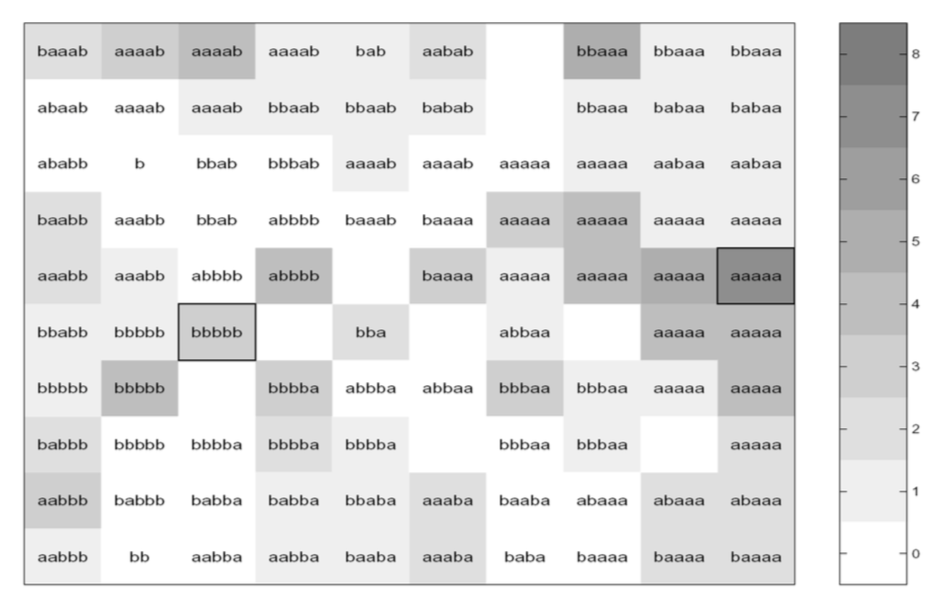
\includegraphics[width=10cm]{assets/receptive_field}
	\caption{Ukážka hitmapy}
\end{figure}

Hĺbku pamäte pre konkrétny neurón v siete vypočítame ako vážený priemer dĺžky najdlhších spoločných 
podpostupností písmen v množine okien vstupov neurónu.
Dĺžku najdlhšej podpostupnosti budem určovať od konca sekvencií v množine. 
Pamäťovú hĺbku siete potom určím ako vážený priemer nameraných pamäťových hĺbok jednotlivých neurónov, kde váhami budú veľkosti
množín.
Priemer pamäťových hĺbok jednotlivých neurónov musí byť vážený, aby neuróny, 
ktoré boli víťazmi pre väčší počet vstupov mali vyššiu váhu ako neuróny, ktoré boli víťazmi pre menší počet vstupov.
Po každej trénovacej epoche (prechode trénovacou množinou) budem vedieť určiť pamäťovú hĺbku mapy.
Vďaka tomu, že neuróny rekurentných sietí majú okrem normálnych váh aj kontextové váhy, 
ktoré uchovávajú informácie z predchádzajúcich krokov, môže sa stať, že rovnaké písmeno zo vstupu 
bude mať rôzne víťazné neuróny počas trénovania.

% do dalsej kapitoly

Samotná pamäťová hĺbka je relatívna a závisí aj od veľkosti posuvného okna (sliding window).
Veľkosť posuvného okna má zmysel zvyšovať iba pokiaľ nám stúpa pamäťová hĺbka, inými
slovami, toto okno musí byť minimálne tak veľké ako je najdlhšia nájdená podpostupnosť v jednotlivých neurónoch.

Počet neurónov v mape volíme podľa množstva rôznych znakov v použitej trénovacej množine.

Tradeoff medzi rozlišovaciou schopnosťou jednotlivých slov a schopnosťou
zachovať podobné slová topologicky čo najbližšie pri sebe.

Na trénovanie a vyhodnocovanie pamäťovej hĺbky som si vytvoril 3 sady 
trénovacích príkladov. 
Prvá sada sú najednoduchšie sekvenice (slová), ktoré obsahujú veľké množstvo regularít a malé množstvo rôznych písmen.
Napríklad sekvencie ako $aaabbb$,  $bbbaaaaa$.
Druhou sadou budú slová generované Reberovým automatom.
Treťou sadou trénovacích príkladov budú najzložitejšie sekvencie, resp. slová z určitého korpusu anglického textu (napríklad úryvok z knihy). 
Túto sadu budem používať ako performance benchmark. 

\section{Hľadanie ideálnych (hyper) parametrov}
Ako prvé je potrebné zvoliť vhodnú veľkosť posuvného okna na trénovacej množine, tak aby bolo väčšie ako
najdlhšia nájdená spoločná podpostupnosť znakov. 
Toto je jednoducho docieliteľné postupným zvyšovaním veľkosti tohto pamäťového okna až pokým pamäťová hĺbka stúpa.

Ďaľšie dôležité parametre, ktoré potrebujem optimalizovať sú $alpha$ a $beta$ parametre, ktoré
sa používajú pri počítaní výslednej vzdialenosti vstupného vektora od váhového vektora neurónu.
Táto vzdialenosť je pri rekurentných SOM určená ako kombinácia vzdialenosti vstupu od váhového vektora neurónu a vzdialenosti
kontextu od contextového vektora neurónu.
Jednotlivé parametre určujú akú váhu má aktuálny vstup a akú váhu má kontext pri výpočte výslednej vzdialenosti.
Toto neviem spraviť nijak inak, iba postupním skúšaním rôznych kombinácii týchto parametrov. 
$alpha$ aj $beta$.

Optimálne $alpha$ a $beta$ parameters, ktoré dávajú najlepšie výsledky som hľadal nasledujúcim
spôsobom:

Naprogramoval som si skript, pomocou ktorého trénujem sieť s rôznymi parametrami.
Výsledky som si počas trénovania zaznamenával.
Následne som si vykreslil 3D grafy pre každý typ trénovanej siete (msom, recsom, vmsom), 
kde na x-ovej osy sú hodnoty alpha parametra, na y-ovej osy sú hodnoty beta parametra a
na z-ovej osy sú hodnoty pamäťových hĺbok.
Na začiatok som zvyšoval parameters po hodnote $0.1$.

% TODO ukazky grafov parametrov pre jednotlive siete







